\chapter{Judges 8}
 
\begin{figure}
  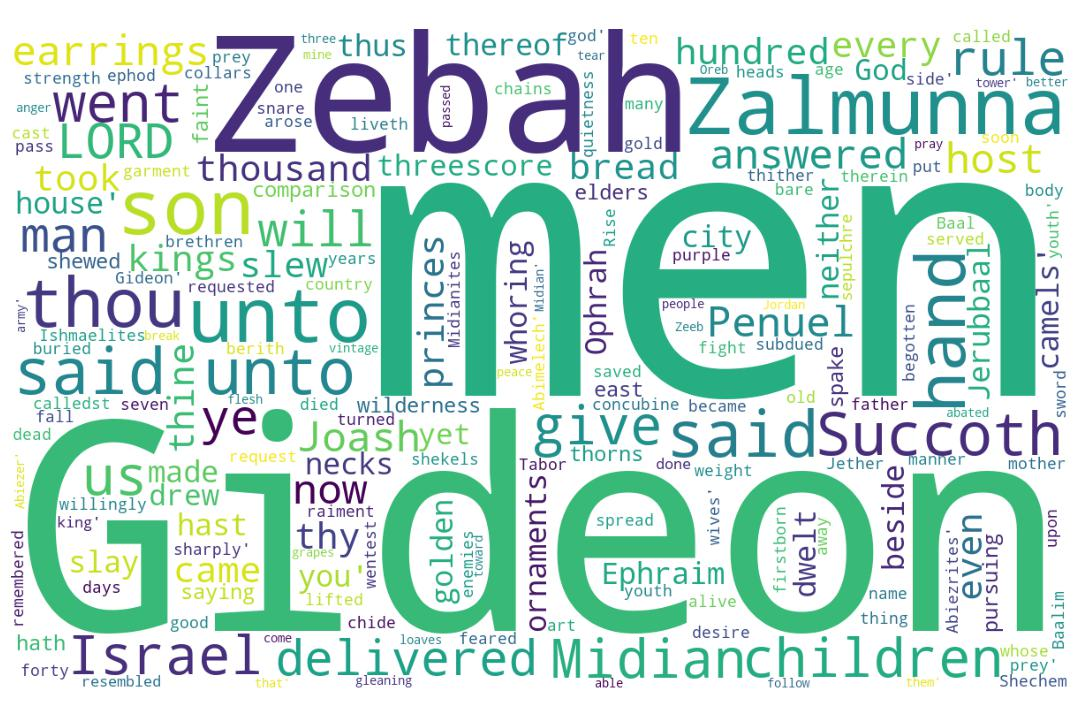
\includegraphics[width=\linewidth]{07OT-Judges/Judges8-WordCloud.jpg}
  \caption{Judges 8 Word Cloud}
  \label{fig:Judges 8 Word Cloud}
\end{figure}


\marginpar{\scriptsize \centering \fcolorbox{bone}{lime}{\textbf{GIDEON'S FAME}}\\ (Judges 8) \begin{compactenum}[I.][8]
    \item \textbf{Made a Hero} \index[scripture]{Judges!Judges 08:12}(Jdg 8:12)
    \item \textbf{Mostly Right} %\index[scripture]{Judges!Judges 07:04}(Judges 7:4)
    \item \textbf{Morally Suspect} \index[scripture]{Judges!Judges 08:24}(Jdg 8:24)
    \item \textbf{Mistreated by the Brethren} \index[scripture]{Judges!Judges 08:06, 08}(Jdg 8:6, 8)
    \item \textbf{Remembered no More} \index[scripture]{Judges!Judges 08:35}(Jdg 8:35)
    \item \textbf{Might in the Flesh} \index[scripture]{Judges!Judges 08:30}(Jdg 8:30)
    \item A \textbf{Momentary Hero} \index[scripture]{Judges!Judges 08:35}(Jdg 8:35)
\end{compactenum}}


\footnote{\textcolor[rgb]{0.00,0.25,0.00}{\hyperlink{JudgesTOC}{Return to end of Table of Contents.}}}\footnote{\href{https://audiobible.com/bible/judges_7.html}{\textcolor[cmyk]{0.99998,1,0,0}{Judges 7 Audio}}}\textcolor[cmyk]{0.99998,1,0,0}{And the men of Ephraim said unto him, Why hast thou served us thus, that thou calledst us not, when thou wentest to fight with the Midianites? And they did chide with him sharply.}
[2] \textcolor[cmyk]{0.99998,1,0,0}{And he said unto them, What have I done now in comparison of you? \emph{Is} not the gleaning of the grapes of Ephraim better than the vintage of Abiezer?}
[3] \textcolor[cmyk]{0.99998,1,0,0}{God hath delivered into your hands the princes of Midian, Oreb and Zeeb: and what was I able to do in comparison of you? Then their anger was abated toward him, when he had said that.}\\
\\
\P \textcolor[cmyk]{0.99998,1,0,0}{And Gideon came to Jordan, \emph{and} passed over, he, and the three hundred men that \emph{were} with him, faint, yet pursuing \emph{them}.}
[5] \textcolor[cmyk]{0.99998,1,0,0}{And he said unto the men of Succoth, Give, I pray you, loaves of bread unto the people that follow me; for they \emph{be} faint, and I am pursuing after Zebah and Zalmunna, kings of Midian.}\\
\\
\P \textcolor[cmyk]{0.99998,1,0,0}{And the princes of Succoth said, \emph{Are} the hands of Zebah and Zalmunna now in thine hand, that we should give bread unto thine army?}
[7] \textcolor[cmyk]{0.99998,1,0,0}{And Gideon said, Therefore when the LORD hath delivered Zebah and Zalmunna into mine hand, then I will tear your flesh with the thorns of the wilderness and with briers.}\\
\\
\P \textcolor[cmyk]{0.99998,1,0,0}{And he went up thence to Penuel, and spake unto them likewise: and the men of Penuel answered him as the men of Succoth had answered \emph{him}.}
[9] \textcolor[cmyk]{0.99998,1,0,0}{And he spake also unto the men of Penuel, saying, When I come again in peace, I will break down this tower.}\\
\\
\P \textcolor[cmyk]{0.99998,1,0,0}{Now Zebah and Zalmunna \emph{were} in Karkor, and their hosts with them, about fifteen thousand \emph{men}, all that were left of all the hosts of the children of the east: for there fell an hundred and twenty thousand men that drew sword.}\\
\\
\P \textcolor[cmyk]{0.99998,1,0,0}{And Gideon went up by the way of them that dwelt in tents on the east of Nobah and Jogbehah, and smote the host: for the host was secure.}
[12] \textcolor[cmyk]{0.99998,1,0,0}{And when Zebah and Zalmunna fled, he pursued after them, and took the two kings of Midian, Zebah and Zalmunna, and discomfited all the host.}\\
\\
\P \textcolor[cmyk]{0.99998,1,0,0}{And Gideon the son of Joash returned from battle before the sun \emph{was} \emph{up},}
[14] \textcolor[cmyk]{0.99998,1,0,0}{And caught a young man of the men of Succoth, and enquired of him: and he described unto him the princes of Succoth, and the elders thereof, \emph{even} threescore and seventeen men.}
[15] \textcolor[cmyk]{0.99998,1,0,0}{And he came unto the men of Succoth, and said, Behold Zebah and Zalmunna, with whom ye did upbraid me, saying, \emph{Are} the hands of Zebah and Zalmunna now in thine hand, that we should give bread unto thy men \emph{that} \emph{are} weary?}
[16] \textcolor[cmyk]{0.99998,1,0,0}{And he took the elders of the city, and thorns of the wilderness and briers, and with them he taught the men of Succoth.}
[17] \textcolor[cmyk]{0.99998,1,0,0}{And he beat down the tower of Penuel, and slew the men of the city.}\\
\\
\P \textcolor[cmyk]{0.99998,1,0,0}{Then said he unto Zebah and Zalmunna, What manner of men \emph{were} \emph{they} whom ye slew at Tabor? And they answered, As thou \emph{art}, so \emph{were} they; each one resembled the children of a king.}
[19] \textcolor[cmyk]{0.99998,1,0,0}{And he said, They \emph{were} my brethren, \emph{even} the sons of my mother: \emph{as} the LORD liveth, if ye had saved them alive, I would not slay you.}
[20] \textcolor[cmyk]{0.99998,1,0,0}{And he said unto Jether his firstborn, Up, \emph{and} slay them. But the youth drew not his sword: for he feared, because he \emph{was} yet a youth.}
[21] \textcolor[cmyk]{0.99998,1,0,0}{Then Zebah and Zalmunna said, Rise thou, and fall upon us: for as the man \emph{is,} \emph{so} \emph{is} his strength. And Gideon arose, and slew Zebah and Zalmunna, and took away the ornaments that \emph{were} on their camels' necks.}\\
\\
\P \textcolor[cmyk]{0.99998,1,0,0}{Then the men of Israel said unto Gideon, Rule thou over us, both thou, and thy son, and thy son's son also: for thou hast delivered us from the hand of Midian.}
[23] \textcolor[cmyk]{0.99998,1,0,0}{And Gideon said unto them, I will not rule over you, neither shall my son rule over you: the LORD shall rule over you.}\\
\\
\P \textcolor[cmyk]{0.99998,1,0,0}{And Gideon said unto them, I would desire a request of you, that ye would give me every man the earrings of his prey. (For they had golden earrings, because they \emph{were} Ishmaelites.)}\
[25] \textcolor[cmyk]{0.99998,1,0,0}{And they answered, We will willingly give \emph{them}. And they spread a garment, and did cast therein every man the earrings of his prey.}
[26] \textcolor[cmyk]{0.99998,1,0,0}{And the weight of the golden earrings that he requested was a thousand and seven hundred \emph{shekels} of gold; beside ornaments, and collars, and purple raiment that \emph{was} on the kings of Midian, and beside the chains that \emph{were} about their camels' necks.}
[27] \textcolor[cmyk]{0.99998,1,0,0}{And Gideon made an ephod thereof, and put it in his city, \emph{even} in Ophrah: and all Israel went thither a whoring after it: which thing became a snare unto Gideon, and to his house.}\\
\\
\P \textcolor[cmyk]{0.99998,1,0,0}{Thus was Midian subdued before the children of Israel, so that they lifted up their heads no more. And the country was in quietness forty years in the days of Gideon.}\\
\\
\P \textcolor[cmyk]{0.99998,1,0,0}{And Jerubbaal the son of Joash went and dwelt in his own house.}
[30] \textcolor[cmyk]{0.99998,1,0,0}{And Gideon had threescore and ten sons of his body begotten: for he had many wives.}\\
\\
\P \textcolor[cmyk]{0.99998,1,0,0}{And Gideon the son of Joash died in a good old age, and was buried in the sepulchre of Joash his father, in Ophrah of the Abiezrites.}
[33] \textcolor[cmyk]{0.99998,1,0,0}{And it came to pass, as soon as Gideon was dead, that the children of Israel turned again, and went a whoring after Baalim, and made Baal-berith their god.}  [34] \textcolor[cmyk]{0.99998,1,0,0}{And the children of Israel remembered not the LORD their God, who had delivered them out of the hands of all their enemies on every side:}
[35] \textcolor[cmyk]{0.99998,1,0,0}{Neither shewed they kindness to the house of Jerubbaal, \emph{namely}, Gideon, according to all the goodness which he had shewed unto Israel.}